\let\negmedspace\undefined
\let\negthickspace\undefined
\documentclass[journal]{IEEEtran}
\usepackage[a5paper, margin=10mm, onecolumn]{geometry}
%\usepackage{lmodern} % Ensure lmodern is loaded for pdflatex
\usepackage{tfrupee} % Include tfrupee package

\setlength{\headheight}{1cm} % Set the height of the header box
\setlength{\headsep}{0mm}     % Set the distance between the header box and the top of the text

\usepackage{gvv-book}
\usepackage{gvv}
\usepackage{cite}
\usepackage{amsmath,amssymb,amsfonts,amsthm}
\usepackage{algorithmic}
\usepackage{graphicx}
\usepackage{textcomp}
\usepackage{xcolor}
\usepackage{txfonts}
\usepackage{listings}
\usepackage{enumitem}
\usepackage{mathtools}
\usepackage{gensymb}
\usepackage{comment}
\usepackage[breaklinks=true]{hyperref}
\usepackage{tkz-euclide} 
\usepackage{listings}
% \usepackage{gvv}                                        
\def\inputGnumericTable{}                                 
\usepackage[latin1]{inputenc}                                
\usepackage{color}                                            
\usepackage{array}                                            
\usepackage{longtable}                                       
\usepackage{calc}                                             
\usepackage{multirow}                                         
\usepackage{hhline}                                           
\usepackage{ifthen}                                           
\usepackage{lscape}
\usepackage{circuitikz}
\tikzstyle{block} = [rectangle, draw, fill=blue!20, 
    text width=4em, text centered, rounded corners, minimum height=3em]
\tikzstyle{sum} = [draw, fill=blue!10, circle, minimum size=1cm, node distance=1.5cm]
\tikzstyle{input} = [coordinate]
\tikzstyle{output} = [coordinate]


\begin{document}

\bibliographystyle{IEEEtran}
\vspace{3cm}

\title{2.4.8}
\author{EE25BTECH11018-Darisy Sreetej}
 \maketitle
% \newpage
% \bigskip
{\let\newpage\relax\maketitle}

\renewcommand{\thefigure}{\theenumi}
\renewcommand{\thetable}{\theenumi}
\setlength{\intextsep}{10pt} % Space between text and floats


\numberwithin{equation}{enumi}
\numberwithin{figure}{enumi}
\renewcommand{\thetable}{\theenumi}

\textbf{Question}:
Find a unit vector perpendicular to each of the vectors $\myvec{\vec{a}+\vec{b}}$ and $\myvec{\vec{a}+\vec{b}}$ where, $\vec{a} = \hat{i} + \hat{j} + \hat{k}$ and $\vec{b} = \hat{i} + 2\hat{j} + 3\hat{k} $ is

\quad

\textbf{Solution}: \\
Given two vectors,\\
\begin{align}
    \vec{a}=\myvec{1\\1\\1} \;\;\; \vec{b}=\myvec{1\\2\\3}
\end{align}
Let the desired vector be $\vec{x}$.
Then,
$\vec{x}=\myvec{x_1 \\
x_2\\
x_3}$
\begin{align}
\myvec{\vec{a}+\vec{b}}=\myvec{\vec{a}&\vec{b}}\myvec{1\\1}
\end{align}
\begin{align}
\myvec{\vec{a}-\vec{b}}=\myvec{\vec{a}&\vec{b}}\myvec{1\\-1}
\end{align}
According to the given question ,
\begin{align}
    \therefore \myvec{\vec{a}+\vec{b}&\vec{a}-\vec{b}}^T\vec{x}=0
\end{align}
(0.4) can be expressed as
\begin{align}
    \cbrak{{\myvec{\vec{a}&\vec{b}}\myvec{1&&1\\1&&-1}}}^T\vec{x}=0
    \end{align}
    \begin{align}
       \myvec{1&&1\\1&&-1}^T \myvec{\vec{a}&\vec{b}}^T\vec{x}=0
    \end{align}
    \begin{align}
         \myvec{1&&1\\1&&-1}\myvec{1&&1\\1&&-1}^T \myvec{\vec{a}&\vec{b}}^T\vec{x}=0
    \end{align}
    or,
    \begin{align}
        \myvec{\vec{a}&\vec{b}}^T\vec{x}=0
    \end{align}
which can be expressed as 
\begin{align}
    \myvec{1&&1&&1\\1&&2&&3}
    \xleftrightarrow{ R_2 = R_2 - R_1}
    \myvec{1&&1&&1\\0&&1&&2}
    \end{align}
    and
    \begin{align}
     \myvec{1&&1&&1\\1&&2&&3}
    \xleftrightarrow{ R_2 = R_2 - 2R_1}
    \myvec{1&&1&&1\\-1&&0&&1}
\end{align}
yielding,
\begin{align}
    x_2+2x_3=0\\
    -x_1+x_3=0
\end{align}
\begin{align}
    \vec{x}=x_3\myvec{1\\-2\\1}
\end{align}
The unit vector is 
\begin{align}
      \vec{x}=\frac{1}{\sqrt{6}}\myvec{1\\-2\\1}
\end{align}
As we know that the vector can be in both the directions i.e, into and out of the plane containing $\vec{a}$ and $\vec{b}$, so the vector perpendicular to vectors $\vec{a}$ and $\vec{b}$ would be $\pm\;(\vec{a} \times \vec{b})$.

\quad 

Therefore, the desired output is
\begin{align}
    \vec{x}=\pm\frac{1}{\sqrt{6}}\myvec{1\\-2\\1}
\end{align}

\newpage

 \begin{figure}
    \centering
    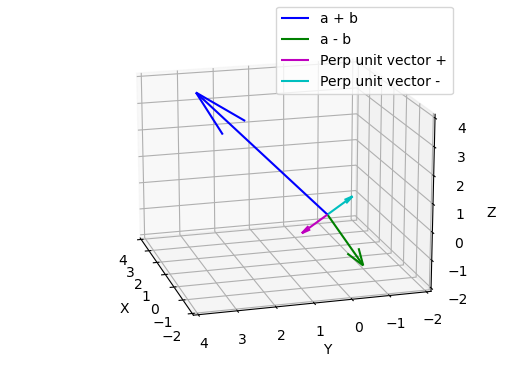
\includegraphics[width=\columnwidth]{figs/fig.png}
    \caption*{The perpendicular unit vectors}
    \label{fig:fig}
\end{figure}



\end{document}
